
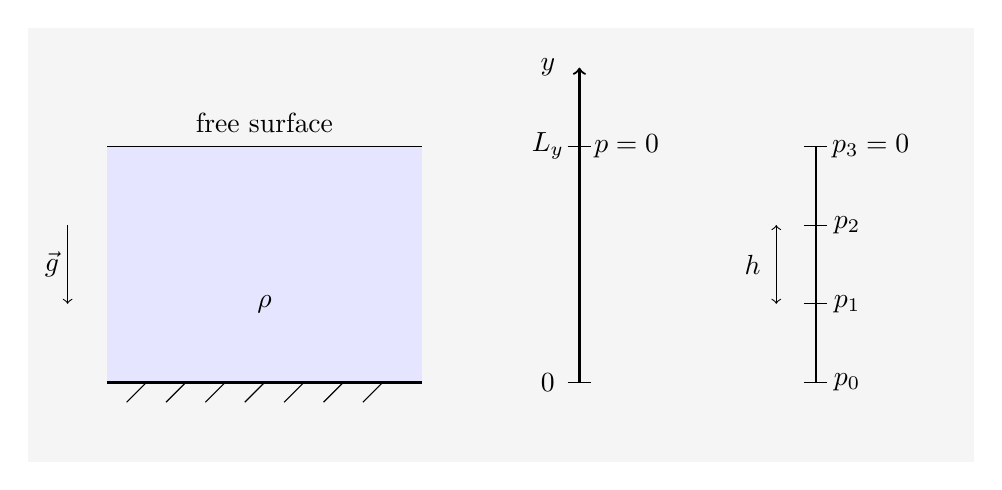
\begin{tikzpicture}
\draw[fill=gray!8,gray!8](0,0) rectangle (12,5.5);
%\draw[step=0.5cm,gray,very thin] (0,0) grid (12,5.5); %background grid

\fill[blue!10!white] (1,1) rectangle (5,4);
\draw[thick,-] (1,1) -- (5,1) ; 
\draw[-] (1,4) -- (5,4) ; 
\draw[->] (0.5,3) -- (0.5,2) ; 
\node[] at (0.3,2.5) {$\vec{g}$};
\node[] at (3,2) {$\rho$};
\node[] at (3,4.3) {free surface};

\draw[-] (1.5,1) -- (1.25,0.75) ; 
\draw[-] (2,1) -- (1.75,0.75) ; 
\draw[-] (2.5,1) -- (2.25,0.75) ; 
\draw[-] (3,1) -- (2.75,0.75) ; 
\draw[-] (3.5,1) -- (3.25,0.75) ; 
\draw[-] (4,1) -- (3.75,0.75) ; 
\draw[-] (4.5,1) -- (4.25,0.75) ; 

%---------------------------------

\draw[thick,->] (7,1) -- (7,5) ; 
\node[] at (6.6,4) {$L_y$};
\node[] at (6.6,1) {$0$};
\draw[-] (6.85,1) -- (7.15,1) ; 
\draw[-] (6.85,4) -- (7.15,4) ; 
\node[] at (7.6,4) {$p=0$};
\node[] at (6.6,5) {$y$};

%---------------------------------

\draw[thick] (10,1) -- (10,4) ; 
\draw[-] (9.85,1) -- (10.15,1) ; 
\draw[-] (9.85,2) -- (10.15,2) ; 
\draw[-] (9.85,3) -- (10.15,3) ; 
\draw[-] (9.85,4) -- (10.15,4) ; 
\node[] at (10.7,4) {$p_3=0$};
\node[] at (10.4,3) {$p_2$};
\node[] at (10.4,2) {$p_1$};
\node[] at (10.4,1) {$p_0$};

\draw[<->] (9.5,2) -- (9.5,3) ;  
\node[] at (9.2,2.5) {$h$};
\end{tikzpicture}


